\section{Architectures and demonstrated capabilities}\label{sec:architectures}

In the literature we examined, multispectral sensor chips and smartphone grating spectrometers are the most common hardware families, with LED photometers and colorimeters close behind; integrated modules, dedicated camera instruments, and other designs appear much less often (Table~\ref{tab:valpractice}). Each publication was counted once, according to its main assembly, and this includes papers that compare several instruments or revisit an existing platform. We grouped RGB sensors and camera photometers without a grating with the LED photometers, whereas dedicated wavelength-selective chips form a family of their own. A system in which a phone controls a separate camera still counts as phone-based, but a computer used only to read out a module does not change the module's family.

Figure~\ref{fig:archschem} sketches a typical transmission layout for each family, with the sample placed outside the integrated detector or module. These layouts are only common arrangements; some colorimeters select their bands at the detector instead, and some smartphone systems use a separate camera.

\begin{figure}[!htbp]
\centering
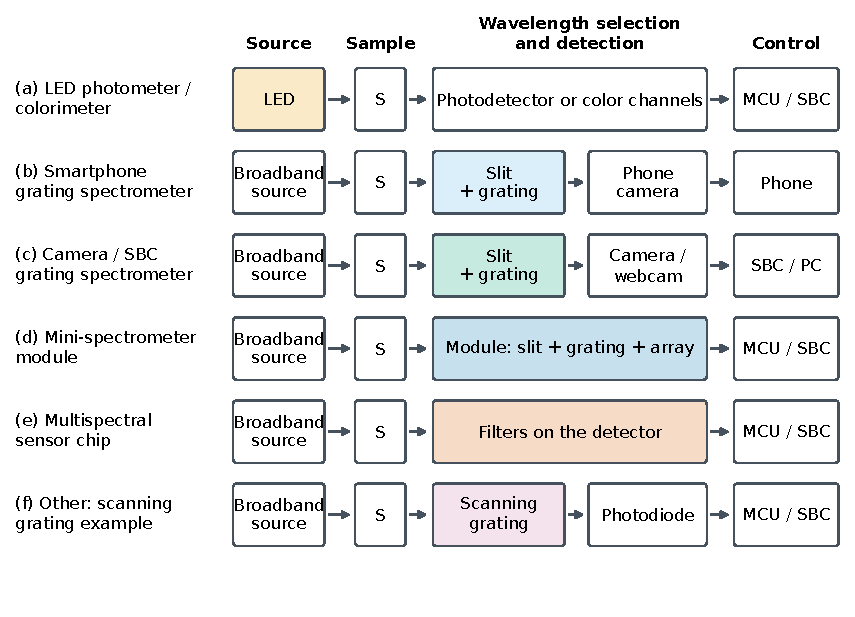
\includegraphics[width=\linewidth, draft=false]{architectures.pdf}

\caption{\FigureCaptionTwo}\label{fig:archschem}
\end{figure}

\subsection{LED photometers and colorimeters}

Instruments built around LEDs keep the optics to a bare minimum for a well-defined assay. The LED is paired with a photodiode,\citep{prairie2020accurate,glotz2018design} a phototransistor, a light-to-frequency converter, or an ambient-light sensor.\citep{nonno2022portuino,wittbrodt2015open,cirrone2025low} RGB sensors\citep{morais2015low,dewantara2023low,fernandes2023portable} and cameras without gratings\citep{tonelli2021sensing,chang2012smartphone} can serve as detectors instead. Because the emitters are interchangeable, a single instrument can handle several assays,\citep{jesus2025modular,konnel2025low} and reported applications run from UV protein measurements through visible-range chemistry to NIR screening of fuels.\citep{poh2021spectrophotometer,prairie2020accurate,dantas2017inexpensive} By combining absorbances at selected wavelengths, a six-channel LED/photodiode instrument detected and quantified synthetic hemozoin in diluted blood.\citep{catarino2020portable}

Calibration can absorb differences in sensitivity between instruments. Two LED units measured iron with sensitivities of 0.136--0.169~L/mg, compared with 0.165--0.180~L/mg for commercial instruments. Relative to the reference instruments, the reported mean sensitivities were 87.7\%, 65.2\%, and 67.0\% for iron, manganese, and fluoride, and yet recoveries in calibration checks were 98.3--104.0\%.\citep{prairie2020accurate} Selectivity is another matter: it still depends on the reagent chemistry, and on the sample matrix when absorption bands overlap.\citep{clippard2016construction,jesus2025modular,cirrone2025low}

Wavelength claims call for particular care when emitters are mixed. Combining red, green, and blue light can reproduce a color, but it does not make a monochromatic source; one assay reported at 412~nm was run on a device whose shortest emission peak lay at 458~nm.\citep{kerestes2023affordable}
